%!TEX root = ./template-skripsi.tex
%-------------------------------------------------------------------------------
%                            BAB II
%               TINJAUAN PUSTAKA DAN DASAR TEORI
%-------------------------------------------------------------------------------

\chapter{TINJAUAN PUSTAKA DAN LANDASAN TEORI}                

\section{Tinjauan Pustaka}
  Penelitian yang dilakukan oleh Alhadi (2013) yang bertujuan merancang sistem informasi penggajian dan pengupahan dengan analisis data dan proses bisnis yang ada pada Bagian Sumber Daya dan Umum PT. Krakatau Wajatama Cilegon, Banten. Hasil yang diperoleh adalah sistem menjadi mudah untuk dipelihara dan dikembangkan, dan mampu mengurangi resiko terjadinya masalah dalam hal pengembangan dan perbaikan sistem yang disebabkan oleh pergantian pengembang sistem.

  Penelitian yang dilakukan oleh Dewanto (2013) yang dilakukan di penerbit buku pendidikan Deepublish Yogyakarta. Penelitian tersebut menghasilkan paket sistem informasi untuk menghitung \emph{cost of production} (biaya produksi) dan penggajian karyawan serta memudahkan dalam perhitungannya serta evaluasi keungan secara berkala.

  Penelitian yang dilakukan oleh Firdaus (2017) yang bertujuan merancang aplikasi sistem informasi penggajian di CV. Sogan Jaya Abadi. \emph{Output} yang dihasilkan adalah proses penggajian karyawan lebih cepat dan akurat serta pengaksesan informasi bisa dilakukan dimanapun dan kapanpun.
  
  Penelitian yang dilakukan oleh Hutama (2016) yang bertujuan untuk merancang perangkat lunak berbasis Android untuk digitalisasi presensi karyawan di PT. Geschool Cerdas Mandiri. Hasil dari penelitian ini adalah perangkat lunak yang dirancang dapat digunakan untuk melakukan manajemen data jam kerja karyawan.
  
  Berdasarkan hasil dari penelitian yang telah disebutkan diatas, \emph{output} yang dihasilkan dan metode yang digunakan dalam pengembangan berbeda-beda. Perbedaan penelitian ini dengan penelitian sebelumnya adalah sistem yang dikembangkan ini memiliki fungsionalitas yang cukup lengkap dengan berbagai aktor yang terlibat dalam pengolahan datanya sesuai dengan hak akses atau wewenang masing-masing aktor. Detail perbandingan penelitian terdahulu yang dijadikan sebagai tinjauan pustaka dapat dilihat pada Tabel.
  \begin{spacing}{1.25}
  \begin{longtable}{|>{\centering}p{1.5em}|p{2cm}|>{\raggedright}p{3cm}|p{3cm}|>{\raggedright}p{4cm}|}
  \caption{Perbedaan Penelitian.}
  \label{perbandingan} \\
  \hline \textbf{No.} & \textbf{Peneliti} & \textbf{Domain} & \textbf{Metode Pengembangan} & \textbf{Hasil}  \\ \hline
  \endfirsthead
  \multicolumn{5}{c}%
  {{\bfseries \tablename\ \thetable{}:} Perbandingan Penelitian (lanjutan)} \\
  \hline \textbf{No.} & \textbf{Peneliti} & \textbf{Domain} & \textbf{Metode Pengembangan} & \textbf{Hasil}  \\ \hline
  \endhead
  \hline
  \endfoot
  \hline \hline
  \endlastfoot
  1. & Alhadi (2013) & Penggajian dan pengupahan karyawan & SDLC & Sistem penggajian dan pengupahan yang termodulisasi, memiliki standar aturan dalam proses pengembangan program \\ \hline
  2. & Dewanto (2013) & \emph{Cost of Production} (COP) dan penggajian karyawan & \emph{Prototyping} & Sistem informasi yang dapat membantu dalam menghitung total gaji berdasar kriteria yang terkait dan perhitungan biaya produksi yang mencakup pengolahan waktu produksi, biaya proses produksi \\ \hline
  3. & Firdaus (2017) & Penggajian karyawan & \emph{Prototyping} & Hak akses pengguna sistem ada empat, yaitu \emph{superadmin}, \emph{hrd}, \emph{finance}, dan direktur perusahaan dengan tujuan utama untuk memaksimalkan proses manajemen karyawan dan penggajian karyawan \\ \hline
  4. & Hutama (2016) & Presensi karyawan & \emph{Extreme Programming} & Aplikasi presensi berbasis android yang memiliki fitur sebagai alat presensi, mengirim permintaan izin, dan melihat laporan presensi \\ \hline
  5. & Usulan (2018) & Penggajian Karyawan & \emph{Extreme Programming} & Sistem informasi penggajian karyawan berbasis web yang dalam pengembangannya melalui beberapa siklus dan dapat menyesuaikan kebutuhan \emph{project owner} agar dihasilkan sistem yang tepat guna dan dapat mambantu dan memudahkan proses penggajian karyawan  \\ \hline
  \end{longtable}
  \end{spacing}
  \vspace{4mm}
  
\section{Landasan Teori}

\subsection{Sistem Informasi}

    \subsubsection{Pengertian Sistem}
    Sistem didefinisikan ke dalam dua kelompok pendekatan, yaitu pendekatan yang menekankan pada prosedurnya dan pendekatan yang menekankan pada komponen dan elemennya. Menurut Jerry FitzGeral dalam bukunya yang berjudul \emph{Fundamentals of Systems Analysis} (1981) mendefinisikan pendekatan sistem yang lebih menekankan pada prosedurnya adalah suatu jaringan kerja dari prosedur-prosedur yang saling berhubungan, berkumpul bersama-sama untuk melakukan suatu kegiatan atau untuk menyelesaikan suatu sasaran yang tertentu. Sedangkan pendekatan yang menekankan pada komponen atau elemennya menyebutkan bahwa sistem adalah kumpulan komponen yang saling berkaitan dan bekerjasama untuk mencapai suatu tujuan tertentu (Ladjamudin, 2005).
    
    \subsubsection{Karakteristik Sistem}
    Untuk membedakan suatu sistem dengan sistem yang lainnya, maka diperlukan sekumpulan karakteristik pada sistem tersebut (Ladjamudin, 2005). Berikut merupakan beberapa karakteristik sistem:
    \begin{enumerate}
        \itemsep0em
        \item Batasan Sistem (\emph{Boundary})
        
        Daerah yang membataskan satu sistem dengan sistem yang lain maupun dengan lingkungan luar dan menunjukan ruang lingkup dari sistem tersebut.
        \item Lingkungan Luar Sistem (\emph{Environment})
        
        Segala sesuatu yang berada di luar sistem yang mempengaruhi operasi sistem. Lingkungan luar sistem dapat bersifat positif (menguntungkan) maupun negatif (merugikan).
        \item Masukan Sistem (\emph{Input})
        
        Energi yang dimasukan ke dalam sistem, dapat berupa perawatan (\emph{maintenance input}) dan masukan sinyal (\emph{signal input}). \emph{Maintenance input} adalah energi yang dimasukan agar sistem tersebut dapat berjalan. \emph{Signal input} adalah enegi yang diproses untuk menghasilkan keluaran (\emph{output}).
        \item Keluaran Sistem (\emph{Output})
        
        Keluaran adalah hasil dari energi yang telah diolah, dapat diklasifikasikan menjadi keluaran yang berguna dan sisa pembuangan. Keluaran dapat merupakan masukan untuk subsistem lain.
        \item Komponen Sistem (\emph{Component})
        
        Suatu sistem terdiri dari beberapa komponen yang saling berinteraksi, saling kerjasama membentuk suatu kesatuan. Komponen atau elemen-elemen dalam sistem ini dapat berupa subsistem ataupun bagian-bagian dari sistem.
        \item Penghubung Sistem (\emph{Interface})
        
        Penghubung merupakan media yang menghubungkan antara satu subsistem dengan subsitem lainnya, melalui penghubung ini memungkinkan sumber-sumber daya mengalir dari satu subsistem ke subsistem lainnya.
        \item Proses Sistem (\emph{Process})
        
        Proses sistem merupakan tempat pengolahan masukan (\emph{Input}) menjadi keluaran (\emph{Output}).
        \item Sasaran dan Tujuan Sistem
        
        Suatu sistem memiliki suatu tujuan atau sasaran. Tanpa adanya tujuan atau sasaran maka operasi sistem tidak akan berarti.
    \end{enumerate}
    
    \subsubsection{Pengertian Data dan Informasi}
    Dalam Ladjamudin (2005), data merupakan kenyataan yang menggambarkan suatu kejadian-kejadian dan kesatuan nyata. Sedangkan menurut Haryanto (2004), data adalah rekaman mengenai fenomena / fakta yang ada atau sedang terjadi. Dari dua definisi tersebut penulis dapat menyimpulkan bahwa data merupakan fakta dari sesuatu atau kejadian yang kita hadapi.

    Menurut Jogiyanto (2005) informasi adalah data yang diolah menjadi bentuk yang lebih berguna dan lebih berarti bagi yang menerimanya. Adapun Davis dalam (Ladjamudin, 2005) mendefinisikan informasi sebagai data yang telah diolah menjadi bentuk yang lebih berarti dan berguna bagi penerimanya untuk mengambil keputusan masa kini maupun yang akan datang. Dari dua definisi di atas penulis dapat menyimpulkan bahwa pengertian informasi adalah data yang telah diolah menjadi bentuk yang lebih berguna dan dapat memberikan nilai bagi penerimanya.

    \subsubsection{Pengertian Sistem Informasi}
    Menurut Leitch dan Davis, sistem informasi adalah suatu sistem di dalam suatu orgasisasi yang mempertemukan kebutuhan pengolahan transaksi, mendukung operasi, bersifat \emph{managerial} dan kegiatan strategi dari suatu organisasi dan menyediakan pihak luar tertentu dengan laporan-laporan yang diperlukan (Jogiyanto, 2005). Sedangkan dalam Whitten (2006), sistem Informasi adalah sekelompok elemen-elemen dalam suatu organisasi yang saling berintegrasi dengan menggunakan masukkan, proses dan keluaran dengan maksud yang sama untuk mencapai suatu tujuan dan dapat digunakan untuk membantu pengambilan keputusan yang tepat.
    
    Dari dua definisi di atas, penulis menyimpulkan bahwa sistem informasi adalah suatu sistem yang menyediakan informasi untuk manajemen dalam mengambil keputusan dan juga untuk menjalankan operasional perusahaan, di mana sistem tersebut merupakan kombinasi dari orang-orang, teknologi informasi dan prosedur-prosedur yang tergorganisasi.
    
    \subsubsection{Komponen Sistem Informasi}
    Sistem informasi memiliki beberapa komponen tertentu (Ladjamudin, 2005), yang diklasifikasikan sebagai berikut:
        \begin{enumerate}
            \itemsep0em
            \item \emph{Hardware} dan \emph{software} berperan sebagai mesin;
            \item \emph{People} (manusia) merupakan pengguna mesin;
            \item \emph{Procedures} yaitu tatacara penggunaan mesin;
            \item Data yang merupakan penghubung antara manusia dan mesin agar terjadi proses pengolahan data.
        \end{enumerate}

\subsection{Konsep Basis Data}

    \subsubsection{Basis Data (\emph{Database})}
    Basis data adalah suatu pengorganisasian sekumpulan data yang saling terkait sehingga memudahkan aktivitas untuk memperoleh informasi. Basis data dimaksudkan untuk mengatasi masalah pada sistem yang memakai pendekatan berbasis berkas (Kadir, 2003).

    Tujuan awal dan utama dalam pengolahan data pada sebuah basis data adalah agar dapat mencari data dengan mudah dan cepat. Di samping itu, pemanfaatan data untuk pengolahan data juga memiliki tujuan-tujuan tertentu. Pemanfaatan basis data dilakukan untuk memenuhi sejumlah tujuan sebagai berikut (Kadir, 2003):
    \begin{enumerate}
      \itemsep0em
      \item Kecepatan dan kemudahan (\emph{Speed})

      Pemanfaatan basis data memungkinkan untuk dapat menyimpan data atau melakukan perubahan/ manipulasi terhadap data atau menampilkan kembali data tersebut dengan cepat dan mudah.
      \item Efisiensi ruang penyimpanan (\emph{Space})

      Penggunaan ruang penyimpanan di dalam basis data dilakukan untuk mengurangi jumlah \emph{redudansi} (pengulangan) data, baik dengan melakukan penerapan sejumlah pengkodean atau dengan membuat relasi-relasi (dalam bentuk \emph{file}) antar kelompok data yang saling berhubungan.
      \item Keakuratan (\emph{Accuracy})

      Pemanfaatan pengkodean atau pembentukan relasi antar data bersama dengan penerapan aturan/ batasan tipe data, domain data, keunikan data dan sebagainya dan diterapkan dalam basis data, sangat berguna untuk menentukan keakuratan pemasukan atau penyimpanan data.
      \item Ketersediaan (\emph{Availability})

      Pertumbuhan data (baik dari jumlah maupun jenisnya) sejalan dengan waktu akan semakin membutuhkan ruang penyimpanan yang besar. Data yang sudah jarang atau bahkan tidak pernah lagi digunakan dapat diatur untuk dilepaskan dari sistem basis data dengan cara penghapusan atau dengan memindahkannya ke media penyimpanan.
      \item Kelengkapan (\emph{Completeness})

      Lengkap atau tidaknya data yang dikelola bersifat relatif baik terhadap kebutuhan pemakai maupun terhadap waktu. Dalam sebuah basis data, struktur dari basis data tersebut juga harus disimpan. Untuk mengakomodasi kebutuhan kelengkapan data yang semakin berkembang, maka tidak hanya menambah \emph{record-record} data, tetapi juga melakukan penambahan struktur dalam basis data.
      \item Keamanan (\emph{Security})

      Sistem keamanan digunakan untuk dapat menentukan siapa saja yang boleh menggunakan basis data dan menentukan jenis operasi apa saja yang boleh dilakukan.
      \item Kebersamaan pemakai

      Pemakai basis data sering kali tidak terbatas hanya pada satu pemakaian saja atau oleh satu sistem aplikasi saja. Basis data yang dikelola oleh sistem (aplikasi) yang mendukung lingkungan \emph{multiuser}, akan dapat memenuhi kebutuhan ini, tetapi dengan menjaga/menghindari terhadap munculnya persoalan baru seperti inkonsistensi data (karena data yang sama diubah oleh banyak pemakai pada saat bersamaan).
    \end{enumerate}

    \subsubsection{DBMS (\emph{Database Management System})}
    DBMS (\emph{Database Management System}) merupakan koleksi terpadu dari \emph{database} dan program-program komputer yang digunakan untuk mengakses dan memelihara \emph{database}. Program-program tersebut menyediakan berbagai fasilitas operasi untuk memasukkan, melacak, dan memodifikasi data kedalam \emph{database}, mendefinisikan data baru, serta mengolah data menjadi informasi yang dibutuhkan (Ladjamudin, 2005).

    Tujuan utama DBMS adalah menyediakan lingkungan yang nyaman dan efisien untuk penyimpanan dan pengambilan data dari basis data. DBMS berperan memberi abstraksi data tingkat tinggi ke pemakai. Sedangkan tujuan lain dari DBMS antara lain (Hariyanto, 2004):
    \begin{enumerate}
      \itemsep0em
      \item Menghindari redudansi dan inkonsistensi data;
      \item Menghindari kesulitan pengaksesan data;
      \item Menghindari isolasi data;
      \item Menghindari terjadinya anomali pengaksesan konkuren;
      \item Menghindari masalah-masalah keamanan;
      \item Menghindari masalah-masalah integritas.
    \end{enumerate}
    
\subsection{Analisa dan Perancangan Sistem}
    Menurut Whitten (2004), analisa sistem adalah teknik pemecahan masalah dengan cara memecahkan sistem ke dalam komponen-komponen dengan tujuan mempelajari komponen tersebut bekerja dan berinteraksi untuk menyelesaikan tujuan mereka. Perancangan sistem merupakan pelengkap dari analisa sistem ke dalam suatu sistem yang utuh dengan tujuan mendapatkan sistem yang lebih baik.

    Ada enam tahap analisis sistem menurut Whitten (2004), yaitu:
    \begin{enumerate}
      \itemsep0em
      \item Menggunakan penelitian sistem;
      \item Mengorganisasikan tim proyek;
      \item Mendefinisikan kebutuhan informasi;
      \item Mendefinisikan kriteria kinerja sistem;
      \item Menyiapkan usulan rancangan;
      \item Menyetujui atau menolak rancangan proyek.
    \end{enumerate}

    Perancangan sistem adalah penentuan proses dan data yang diperlukan oleh sistem baru, jika sistem itu berbasis komputer, perancangan dapat menyertakan spesifikasi peralatan yang akan digunakan (McLeod, 2001).

    Adapun tahapan perancangan sistem sebagai berikut:
    \begin{enumerate}
      \itemsep0em
      \item Menyiapkan rancangan sistem yang terperinci;
      \item Mengidentifikasi berbagai alternatif sistem;
      \item Mengevaluasi berbagai alternatif konfigurasi sistem;
      \item Memilih konfigurasi terbaik;
      \item Menyiapkan usulan penerapan;
      \item Menyetujui atau menolak penerapan sistem.
    \end{enumerate}

    Dari berbagai penjelasan di atas, penulis dapat menyimpulkan bahwa analisa dan perancangan sistem adalah proses dimana menerjemahkan kebutuhan pemakai informasi ke dalam sebuah rancangan guna memenuhi kebutuhan dari pemakai informasi dan memberikan gambaran yang lebih jelas untuk dijadikan pertimbangan.
    
  \subsection{Gaji}
    \subsubsection{Pengertian Gaji}
    Gaji adalah balas jasa dalam bentuk uang yang diterima karyawan sebagai konsekuensi dan statusnya sebagai seorang karyawan yang memberikan kontribusi dalam mencapai tujuan perusahaan. Sedangkan menurut Rivai dan Sagala (2009), gaji dapat juga diartikan sebagai bayaran tetap yang diterima seseorang karena kedudukannya dalam perusahaan.
    
    \subsubsection{Tujuan Pemberian Upah dan Gaji}
    Berikut adalah tujuan dalam pemberian upah dan gaji (Rivai dan Sagala, 2009):
    \begin{enumerate}
        \itemsep0em
        \item Ikatan Kerja Sama
        
        Dengan pemberian upah dan gaji terjalinlah ikatan kerja sama formal antara pemilik/ pengusaha dengan karyawan. Karyawan harus mengerjakan tugas-tugasnya dengan baik, sedangkan pemilik wajib membayar upah dan gaji sesuai dengan perjanjian yang disepakati.
        \item Kepuasan Kerja
        
        Dengan upah dan gaji, karyawan akan dapat memenuhi kebutuhan fisik, status sosial, dan egoistiknya sehingga memperoleh kepuasan kerja dari jabatannya.
        \item Pengadaan Efektif
        
        Jika program upah dan gaji ditetapkan cukup besar, pengadaan karyawan yang \emph{qualified} untuk perusahaan akan lebih mudah.
        \item Motivasi
        
        Jika upah dan gaji yang diberikan cukup besar, manajer akan mudah memotivasi karyawannya.
        \item Stabilitas Karyawan
        
        Dengan program upah dan gaji atas prinsip adil dan layak serta eksternal konsistensi yang kompetitif maka karyawan lebih terjamin \emph{turnover} relatif kecil.
        \item Disiplin
        
        Dengan pemberian upah dan gaji yang cukup besar maka disiplin karyawan semakin baik. Mereka akan menyadari serta mentaati peraturan-peraturan yang berlaku.
        \item Pengaruh Serikat Buruh
        
        Dengan program upah dan gaji yang baik, pengaruh serikat buruh dapat dihindarkan dan karyawan akan berkonsentrasi pada pekerjaannya.
        \item Pengaruh Pemerintah
        
        Jika program upah dan gaji sesuai dengan undang-undang perburuhan yang berlaku, maka intervensi pemerintah dapat dihindarkan.
    \end{enumerate}

  \subsection{Insentif}
    \subsubsection{Pengertian Insentif}
    Insentif diartikan sebagai bentuk pembayaran yang dikaitkan dengan kinerja dan \emph{gainsharing}, sebagai pembagian keuntungan bagi karyawan akibat peningkatan produktivitas atau penghemat biaya. Sistem ini merupakan bentuk lain dari kompensasi langsung di luar gaji dan upah yang merupakan kompensasi tetap, yang disebut sistem kompensasi berdasarkan kinerja (Rivai dan Sagala, 2009).
    
    Berdasarkan pengertian di atas, peneliti menyimpulkan bahwa insentif digunakan oleh perusahaan sebagai alat untuk memotivasi karyawan guna mencapai tujuan organisasi. Selain hal itu, pemberian insentif juga merupakan strategi efektif dalam kesuksesan suatu perusahaan.
    
    \subsubsection{Tujuan Insentif}
    Tujuan utama dari insentif adalah untuk memberikan tanggung jawab dan dorongan kepada karyawan dalam rangka meningkatkan kualitas dan kuantitas hasil kerjanya. Sedangkan bagi perusahaan, insentif merupakan strategi untuk meningkatkan produktivitas dan efisiensi perusahaan dalam menghadapi persaiangan yang semakin ketat, dimana produktivitas menjadi satu hal yang sangat penting (Rivai dan Sagala, 2009).
    
\subsection{Kinerja dan Penilaian Prestasi}
Kinerja merupakan suatu fungsi dari motivasi dan kemampuan. Untuk menyelesaikan tugas atau pekerjaan seseorang sepatutnya memiliki derajat kesediaan dan tingkat kemampuan tertentu. Kesediaan dan ketrampilan seseorang tidaklah cukup efektif untuk mengerjakan sesuatu tanpa pemahaman yang jelas tentang apa yang akan dikerjakan dan begaimana mengerjakannya. Kinerja merupakan perilaku nyata yang ditampilkan setiap orang sebagai prestasi kerja yang dihasilkan oleh karyawan sesuai dengan perannya dalam perusahaan. Kinerja karyawan merupakan suatu hal yang sangat penting dalam upaya perusahaan untuk mencapai tujuannya (Rivai dan Sagala, 2009).
    
Instrumen penilaian kinerja dapat digunakan untuk \emph{review} kinerja, peringkat kinerja, penilaian karyawan dan sekaligus evaluasi karyawan sehingga dapat diketahui mana karyawan yang mampu melaksanakan pekerjaan secara baik, efisien, efektif, dan produktif sesuai dengan tujuan perusahaan (Rivai dan Sagala, 2009).

    \subsubsection{Tujuan Penilaian Kinerja}
    Suatu perusahaan melakukan penilaian kinerja didasarkan pada dua alasan pokok, yaitu: (1) manajer memerlukan evaluasi yang objektif terhadap kinerja karyawan pada masa lalu yang akan digunakan untuk membuat keputusan di bidang SDM di masa yang akan datang; dan (2) manajer memerlukan alat yang memungkinkan untuk membantu karyawannya memperbaiki kinerja, merencanakan pekerjaan, mengembangkan kemampuan dan ketrampilan untuk perkembangan karier dan memperkuat kualitas hubungan antarmanajer yang bersangkutan dengan karyawannya (Rivai dan Sagala, 2009).
    
    Selain itu penilaian kinerja dapat digunakan untuk (Rivai dan Sagala, 2009):
    \begin{enumerate}
        \itemsep0em
        \item Mengetahui perkembangan, yaitu meliputi: (a) identifikasi kebutuhan pelatihan, (b) umpan balik kerja, (c) menentukan transfer dan penugasan, dan (d) identifikasi kekuatan dan kelemahan karyawan.
        \item Pengambilan keputusan administratif, yang meliputi: (a) keputusan untuk menentukan gaji, promosi, mempertahankan atau memberhentikan karyawan, (b) pengakuan kinerja karyawan, (c) pemutusan hubungan kerja, dan (d) mengidentifikasi yang buruk.
        \item Keperluan perusahaan, yang meliputi: (a) perencanaan SDM, (b) menentukan kebutuhan pelatihan, (c) evaluasi pencapaian tujuan perusahaan, (d) informasi untuk identifikasi tujuan, (e) evaluasi terhadap sistem SDM, dan (f) penguatan terhadap kebutuhan pengembangan perusahaan.
        \item Dokumentasi, yang meliputi: (a) kriteria untuk validasi penelitian, (b) dokumentasi keputusan-keputusan tentang SDM, dan (c) membantu untuk memenuhi persyaratan hukum.
    \end{enumerate}
    
    \subsubsection{Jenis-jenis Penilaian Kinerja}
    Jenis-jenis penilaian kinerja (Rivai dan Sagala, 2009):
    \begin{enumerate}
        \itemsep0em
        \item Penilaian hanya oleh atasan.
        
        Penilaian ini cepat dan langsung. Dapat mengarah ke distorsi karena pertimbangan pribadi.
        \item Penilaian oleh kelompok lini.
        
        Atasan dan atasannya lagi bersama-sama membahas kinerja dari bawahannya yang dinilai. Objektivitasnya lebih akurat dibandingkan hanya oleh atasan sendiri. Individu yang dinilai tinggi dapat mendominasi penilaian.
        \item Penilaian oleh kelompok staf.
        
        Atasan meminta satu atau lebih individu untuk bermusyawarah dengannya, tetapi atasan langsung yang membuat keputusan akhir. Penilaian ini merupakan penilaian gabungan yang masuk akal dan wajar.
        \item Penilaian melalui keputusan komite.
        
        Sama seperti pada pola sebelumnya kecuali bahwa manajer yang bertanggung jawab tidak lagi mengambil keputusan akhir, tetapi hasilnya didasarkan pada pilihan mayoritas. Penilaian ini memperluas pertimbangan yang ekstrim tetapi memperlemah integritas manajer yang bertanggung jawab.
        \item Penilaian berdasarkan peninjauan lapangan.
        
        Sama seperti pada kelompok staf, namun melibatkan wakil dari pimpinan pengambangan atau departemen SDM yang bertindak sebagai peninjau yang independen. Membawa satu pikiran yang tetap ke dalam suatu penilaian lintas sektor yang besar.
        \item Penilaian oleh bawahan dan sejawat.
        
        Mungkin terlalu subjektif dan digunakan sebagai tambahan pada jenis-jenis penilaian yang lain.
    \end{enumerate}

  \subsection{Pemrograman Web}

    \subsubsection{PHP: Hypertext Preprocessor}
    PHP merupakan bahasa berbentuk skrip yang ditempatkan dalam server dan diproses di server. Secara khusus, PHP dirancang untuk membentuk aplikasi web dinamis, artinya ia dapat membentuk suatu tampilan berdasarkan permintaan terkini. Skrip PHP berkedudukan sebagai \emph{tag} dalam bahasa HTML yang merupakan bahasa standar untuk membuat halaman \emph{web} (Kadir, 2008).

    Salah satu kelebihan dari PHP adalah mampu berkomunikasi dengan berbagai \emph{database} yang dikenal. Dengan demikian, menampilkan data yang bersifat dinamis yang diambil dari \emph{database} merupakan hal yang mudah untuk diimplementasikan. Itulah sebabnya sering dikatakan bahwa PHP sangat cocok untuk membangun halaman-halaman web dinamis (Kadir, 2008).

    \subsubsection{MySQL}
    MySQL dikembangkan oleh sebuah perusahaan Swedia bernama MySQLAB yang pada saat itu bersama TeX Data Consult AB sekitar tahun 1994-1995, namun cikal bakal kodenya sudah ada sejak 1979. Awalnya TeX membuat MySQL dengan tujuan mengembangkan aplikasi web untuk klien. TeX merupakan perusahaan pengembang \emph{software} dan konsultan \emph{database}. Saat ini MySQL sudah diakuisisi oleh Oracle Corp (Arief, 2011).
    
    MySQL adalah salah satu jenis \emph{database} server yang sangat terkenal banyak digunakan untuk membangun aplikasi web yang menggunakan \emph{database} sebagai sumber dan pengolahan datanya. Kepopuleran MySQL antara lain karena MySQL menggunakan SQL sebagai bahasa dasar untuk mengakses \emph{database} sehingga mudah untuk digunakan, kinerja \emph{query} cepat, dan mencukupi untuk kebutuhan \emph{database} perusahaan skala menengah-kecil. MySQL juga bersifat \emph{open source} dan \emph{free} (tidak perlu membayar untuk menggunakannya) pada berbagai \emph{platform} (kecuali pada \emph{Windows} yang bersifat \emph{shareware}). MySQL didistribusikan dengan lisensi \emph{open source} GPL (\emph{General Public License}) mulai versi 3.23, pada bulan Juni 2000 (Arief, 2011).
    
    MySQL termasuk RDBMS (\emph{Relational Database Management System}). Itulah sebabnya istilah tabel, baris, dan kolom digunakan pada MySQL. Pada MySQL, sebuah \emph{database} mengandung satu atau sejumlah tabel. Tabel terdiri atas sejumlah kolom dan baris, di mana setiap kolom berisi sekumpulan data yang memiliki tipe yang sejenis, dan baris merupakan sekumpulan data yang saling berkaitan dan membentuk informasi. Kolom biasanya juga disebut sebagai \emph{field} dan informasi yang tersimpan dalam baris disebut \emph{record} (Arief, 2011).

  \subsection{Framework PHP}

    \subsubsection{Pengertian \emph{Framework}}
    Menurut Hakim (2010), \emph{framework} diartikan sebagai koleksi atau kumpulan potongan-potongan program yang disusun atau diorganisasikan sedemikian rupa, sehingga dapat digunakan untuk membantu membuat aplikasi utuh tanpa harus membuat semua kode programnya dari awal.
    
    \subsubsection{Alasan Menggunakan \emph{Framework}}
    Salah satu alasan mengapa orang menggunakan \emph{framework} terutama dalam membangun sebuah aplikasi adalah kemudahan yang ditawarkan. Di dalam sebuah  \emph{framework} biasanya sudah tersedia struktur aplikasi yang baik, \textbf{\emph{standard coding}} (1), \textbf{\emph{best practice}} (2), \textbf{\emph{design pattern}} (3), dan \textbf{\emph{common function}} (4). Dengan menggunakan \emph{framework} kita dapat langsung fokus kepada \emph{business process} yang dihadapi tanpa harus berfikir banyak masalah struktur aplikasi, standar \emph{coding} dan lain-lain (Daqiqil, 2011).
    
    Dengan memanfaatkan \emph{design pattern} dan \emph{common function} yang telah ada, maka hal tersebut dapat mempercepat proses pengembangan aplikasi. Kita tidak perlu membuat suatu fungsionalitas yang bersifat umum. Tanpa disadari ketika kita membangun sebuah aplikasi yang banyak melibatkan banyak fungsionalitas yang telah dibangun itu ternyata sama atau berulang-ulang. Dengan pengelompokan itulah kita dapat mempercepat pengembangan aplikasi (Daqiqil, 2011).
    
    Selain kemudahan dan kecepatan dalam membangun sistem, dengan mengunakan \emph{framework} tertentu kita juga dapat menyeragamkan cara kita mengimplementasikan kode program. Dengan \emph{framework} kita dipaksa untuk patuh kepada sebuah kesepakatan. Selain itu juga akan memudahkan pengembang lain untuk mempelajari dan mengubah aplikasi yang telah dibuat apabila kode yang dihasilkan konsisten dan patuh pada sebuah aturan tertentu (Daqiqil, 2011).

    \subsubsection{Codeigniter}
    Salah satu \emph{framework} PHP yang tangguh dan populer adalah \emph{Codeigniter}. \emph{Codeigniter} awalnya ditulis oleh Rick Ellis, pendiri dan CEO Ellislab, perusahaan yang mengembangkan \emph{Codeigniter}. Di dalam websitenya, \emph{www.codeigniter.com}, \emph{Codeigniter} merupakan sebuah \emph{framework} untuk web yang dibuat dalam format PHP. Format yang dibuat ini selanjutnya dapat digunakan untuk membuat sistem aplikasi \emph{web} yang sangat kompleks. \emph{Codeigniter} mempercepat proses pembuatan \emph{web}, karena menyediakan berbagai macam \emph{class}, \emph{helper}, dan \emph{library} yang dapat kita gunakan selama pengembangan. Selain itu \emph{codeigniter} juga merupakan \emph{framework} yang bersifat \emph{open source}.
    
    Menurut Daqiqil (2011), \emph{codeigniter} sendiri dibangun menggunakan konsep Model-View-Controller \emph{development pattern}. \emph{Codeigniter} sendiri merupakan salah satu \emph{framework} tercepat dibandingkan dengan \emph{framework} lainnya. Pada acara frOSCon (Agustus 2008), pembuat PHP Rasmus Lerdorf mengatakan menyukai \emph{codeigniter} karena dia lebih ringan dan cepat dibandingkan \emph{framework} lainnya ("\emph{because it is faster, lighter and the least like a framework}").
    
    \emph{Codeigniter} memiliki kelebihan-kelebihan yang bermanfaat, yaitu (Daqiqil, 2011):
    \begin{enumerate}
        \itemsep0em
        \item Menggunakan Pattern MVC. Dengan menggunakan pattern MVC ini, struktur kode yang dihasilkan menjadi lebih terstruktur dan memiliki standar yang jelas
        \item URL Friendly. URL yang dihasilkan sangat \emph{user friendly}
        \item Kemudahan. Kemudahan dalam mempelajari, membuat \emph{library} dan \emph{helper}, memodifikasi serta mengintegrasikan keduanya.
        \item Kecepatan. Berdasarkan hasil \emph{benchmark Codeigniter} merupakan salah satu \emph{framework} PHP tercepat yang ada saat ini.
        \item Mudah dimodifikasi dan beradaptasi. Sangat mudah dimodifikasi \emph{behavior framework} ini. Tidak membutuhkan \emph{server requirement} yang macam-macam serta mudah mengadopsi \emph{library} lainnya.
        \item Dokumentasi lengkap dan jelas. Bahkan tanpa buku, \emph{Codeigniter} sebenarnya telah menyediakan sebuah panduan yang lengkap mengenai \emph{Codeigniter}. Semua informasi yang dibutuhkan ada disana.
        \item Learning Curve rendah. \emph{Codeigniter} sangat mudah dipelajari. Dalam memilih \emph{framework} hal ini sangat penting diperhatikan karena kita juga harus memperhatikan skil dari seluruh anggota tim. Jika sebuah \emph{framework} sangat sulit dipelajari maka akan beresiko memperlambat \emph{team development}.
    \end{enumerate}
    \begin{figure}[H]
        \centering
          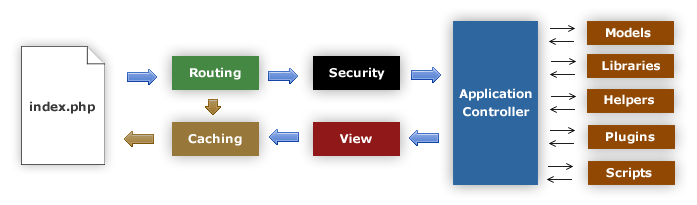
\includegraphics[width=14cm]{gambar/codeigniter}
          \caption{Alur Framework Codeigniter}
          \label{codeigniter}
      \end{figure}
    
    Gambar \ref{codeigniter} menggambarkan bagaimana data mengalir di seluruh sistem \emph{framework Codeigniter}. Kemudian deskripsi alur \emph{framework Codeigniter} dari Gambar \ref{codeigniter} adalah sebagai berikut (Hakim, 2010):
    \begin{enumerate}
      \itemsep0em
      \item Index.php yang berfungsi sebagai kontrol depan, melalui \emph{base} yang dibutuhkan untuk menjalankan \emph{Codeigniter}.
      \item \emph{Router} yang meneliti permintaan HTTP untuk menentukan apa yang harus dilakukan dengannya.
      \item Jika \emph{file cache} ada, maka langsung dikirim ke \emph{browser}.
      \item Sebelum aplikasi kontrol di ambil, maka permintaan HTTP dan pengguna mengirimkan data untuk disaring keamanannya.
      \item \emph{Controller} memanggil \emph{model, core library, plugin, helper} dan \emph{resource} lainnya yang diperlukan untuk memproses permintaan khusus.
      \item \emph{View} yang selesai kemudian dikirim ke \emph{web browser} untuk dilihat.
    \end{enumerate}

  \subsection{\emph{Unified Modeling Language} (UML)}
    \subsubsection{Definisi UML}
    UML merupakan satu kumpulan konvensi pemodelan yang digunakan untuk menentukan atau menggambarkan sebuah sistem \emph{software} yang terkait dengan obyek (Whitten, 2004). UML menawarkan diagram yang dikelompokkan menjadi beberapa perspektif berbeda untuk memodelkan suatu sistem, seperti satu set cetak biru (\emph{blueprint}) yang digunakan untuk membangun sebuah rumah (Whitten, 2004).

    \subsubsection{\emph{Use Case Diagram}}
    \emph{Use Case Diagram} merupakan diagram yang menggambarkan interaksi antara sistem dengan eksternal sistem dan pengguna. Dengan kata lain, secara grafis menggambarkan siapa yang akan menggunakan sistem dan dengan cara apa pengguna mengharapkan untuk berinteraksi dengan sistem (Whitten, 2004).

    Berikut ini merupakan pemodelan yang dimiliki oleh \emph{Use case diagram} (Whitten, 2004): \newline
    \begin{enumerate}
      \itemsep0em
      \item \emph{Use case}
      
      \emph{Use case} merupakan urutan langkah-langkah yang secara tindakan saling terkait (\emph{scenario}), baik otomatis maupun secara manual.
      \item \emph{Actor} (Pelaku)
      
      \emph{Actor} merupakan segala sesuatu yang perlu berinteraksi dengan sistem untuk pertukaran informasi.
      \item \emph{Relationship} (Hubungan)
      
      \emph{Relationship} digambarkan sebagai sebuah garis antara dua simbol. Pemaknaan \emph{relationship} berbeda-beda tergantung bagaimana garis tersebut digambar dan tipe simbol apa yang digunakan untuk menghubungkan garis tersebut. Berikut ini adalah perbedaan di antara \emph{relationship} yang ada pada sebuah diagram \emph{use case}:
        \begin{enumerate}[label=\alph*.]
          \itemsep0em
          \item \emph{Association}
          
          \emph{Association} merupakan \emph{relationship} antara \emph{actor} dengan \emph{use case} dimana terjadi interaksi di antara merekan.
          \item \emph{Extends}
          
          \emph{Extends use case} merupakan \emph{use case} yang terdiri dari langkah yang terekstrasi dari \emph{use case} yang lebih kompleks untuk menyederhanakan masalah dan karena itu memperluas fungsinya.
          \item \emph{Uses} (\emph{includes})
          
          Hubungan \emph{uses} menggambarkan bahwa satu \emph{use case} seluruhnya meliputi fungsionalitas dari \emph{use case} lainnya.
          \item \emph{Depends on}
          
          Terkadang \emph{use case} memiliki ketergantungan pada \emph{use case} lainnya yang bertujuan menentukan urutan dalam pengembangan \emph{use case}. Ketergantungan ini dimodelkan menggunakan \emph{depends on relationship}.
          \item \emph{Inheritance}
          
          Hubungan \emph{inheritance} terjadi ketika dua atau lebih \emph{actor} menggunakan \emph{use case} yang sama.
        \end{enumerate}
    \end{enumerate}

    \subsubsection{\emph{Activity Diagram}}
    \emph{Activity diagram} secara grafis digunakan untuk menggambarkan rangkaian aliran aktifitas baik proses bisnis atau \emph{use case} (Whitten, 2004).

    \subsubsection{\emph{Sequence Diagram}}
    \emph{Sequence diagram} secara grafis menggambarkan bagaimana obyek berinteraksi dengan satu sama lain melalui pesan pada eksekusi sebuah \emph{use case} atau operasi. Diagram ini mengilustrasikan bagaimana pesan terkirim dan diterima di antara obyek dan \emph{sequence} (ruang waktu) (Whitten, 2004).

    \subsubsection{\emph{Class Diagram}}
    \emph{Class Diagram} adalah gambar grafis mengenai struktur obyek statis dari suatu sistem, menunjukan kelas-kelas obyek yang menyusun sebuah sistem dan juga hubungan antara kelas obyek tersebut (Whitten, 2004).

    \subsubsection{Keunggulan UML}
    Adi Nugroho mengemukakan bahwa secara umum UML diterapkan dalam pengembangan sistem atau perangkat lunak beriontasi obyek sebab metodologi UML ini umumnya memiliki keunggulan-keunggulan sebagai berikut (Nugroho, 2005):
    \newline
    \begin{enumerate}
      \itemsep0em
      \item \emph{Uniformity}
      
      Dengan metodologi UML, para pengembang cukup menggunakan satu metodologi dari tahap analisis hingga perancangan. Hal ini tidak bisa dilakukan dalam pengembangan terstruktur. Dengan perkembangan masa kini ke arah aplikasi GUI (\emph{Graphical User Interface}), UML juga memungkinkan kita merancang komponen antar muka pengguna secara integrasi bersama dengan perancangan perangkat lunak sekaligus dengan perancangan basis data.
      \item \emph{Understandability}
      
      Dengan metodologi ini kode yang dihasilkan dapat diorganisasi ke dalam kelas-kelas yang berhubungan dengan masalah sesungguhnya sehingga lebih mudah dipahami oleh siapapun.
      \item \emph{Stability}
      
      Kode program yang dihasilkan relatif stabil sepanjang waktu sebab sangat mendekati permasalahan sesungguhnya di lapangan.
      \item \emph{Reuseability}
      
      Dengan metodologi berorientasi obyek, dimungkinkan penggunaan ulang kode, sehingga pada gilirannya akan sangat mempercepat pengembangan perangkat lunak.
    \end{enumerate}

  \subsection{\emph{Extreme Programming}}
  Permasalahan utama yang sering muncul dalam sebuah proyek pengembangan perangkat lunak adalah perubahan \emph{requirement} yang begitu cepat. Hal ini terjadi sebagai akibat perubahan-perubahan yang muncul baik pada aspek bisnis maupun teknologi yang berlangsung lebih cepat daripada proses pengembangan perangkat lunak itu sendiri. \emph{Extreme Programming} (XP) adalah sebuah pendekatan pengembangan perangkat lunak yang mencoba meningkatkan efisiensi dan fleksibilitas dari sebuah proyek pengembangan perangkat lunak dengan mengkombinasikan berbagai ide sederhana (Widhiartha, 2008).
  
    \begin{figure}[H]
        \centering
        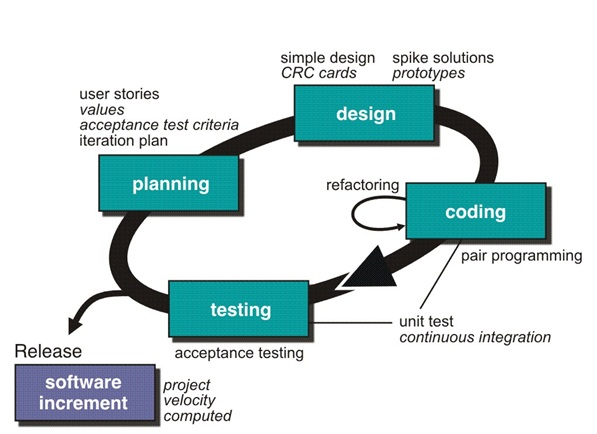
\includegraphics[width=10cm]{gambar/siklus-xp}
        \caption{Siklus \emph{Extreme Programming}}
        \label{siklus_xp}
    \end{figure}
  Menurut Sutabri (2004), \emph{Extreme Programming} terdiri dari aktifitas perencanaan (\emph{planning}), desain (\emph{design}), pengkodean (\emph{coding}), dan pengujian (\emph{testing}). Gambar \ref{siklus_xp} merupakan gambaran dari aktifitas yang ada pada \emph{Extreme Programming}, dan keterangan dari setiap tahapannya adalah sebagai berikut:
  \begin{enumerate}
      \itemsep0em
      \item \emph{Planning}
      
      Tahapan ini dimulai dengan membuat \emph{user story} (cerita) atau gambaran fitur serta fungsi dari sistem yang akan dibangun.
      \item \emph{Design}
      
      Aktifitas desain dalam pengambangan sistem bertujuan untuk merancang pola logika dalam sistem. Desain dibuat berdasarkan \emph{user story} sebelumnya.
      \item \emph{Coding}
      
      Tahap pembuatan sistem berdasarkan \emph{design} yang telah dibuat. Tahap ini dapat dilakukan secara berulang-ulang (\emph{refactoring}) apabila terdapat koreksi dari tahap berikutnya.
      \item \emph{Testing}
      
      Tahap pengujian sistem, setiap modul yang sedang dikembangkan akan terlebih dahulu mengalami pengujian. Apabila masih belum sesuai dengan permintaan maka akan dilakukan perbaikan pada bagian yang dikoreksi. Jika sudah sesuai dengan permintaan maka sistem sudah dapat diimplementasikan.
  \end{enumerate}
  \subsubsection{Nilai-nilai Dasar \emph{Extreme Programming}}
  Berikut adalah nilai-nilai mendasar yang menjadi roh dari XP pada setiap tahapan proses pengembangan perangkat lunak (Widhiartha, 2008):
  \begin{enumerate}
      \itemsep0em
      \item \emph{Communication}
      
      XP mengfokuskan pada hubungan komunikasi yang baik antar anggota tim. Para anggota tim harus membangun saling pengertian, mereka juga wajib saling berbagi pengetahuan dan keterampilan dalam mengembangkan perangkat lunak. Ego dari para programer yang biasaanya cukup tinggi harus ditekan dan mereka harus membuka diri untuk bekerjasama dengan programer lain dalam menuliskan kode program. \newline
      \item \emph{Courage}
      
      Para anggota tim dan penanggungjawab pengembangan perangkat lunak harus selalu memiliki keyakinan dan integritas dalam melakukan tugasnya. Integritas ini harus selalu dijaga bahkan dalam kondisi adanya tekanan dari situasi sekitar.
      \item \emph{Simplicity}
      
      Lakukan semua dengan sederhana. Gunakan \emph{method} yang pendek dan simpel, jangan terlalu rumit dalam membuat desain, hilangkan fitur yang tidak ada gunanya, dan berbagai proses penyederhanaan lain akan selalu menjadi nilai utama dari setiap aspek XP.
      \item \emph{Feedback}
      
      Berikan selalu \emph{feedback} kepada sesama anggota tim maupun pihak lain yang terlibat dalam pengembangan. Utarakan selalu pikiran dan diskusikan kesalahan-kesalahan yang muncul selama proses pengembangan. \emph{Feedback} inilah yang membuat kita menyadari bagian mana yang salah atau bisa ditingkatkan lagi.
      \item \emph{Quality Work}
      
      Dari ke empat nilai yang telah dijelaskan, maka akan berujung pada sebuah kondisi dimana kita melakukan pekerjaan dengan berkualitas. Dengan proses yang berkualitas maka implikasinya akan muncul pula perangkat lunak yang berkualitas sebagai hasil akhirnya.
  \end{enumerate}
  
  \subsubsection{Aspek Dasar \emph{Extreme Programming}}
  Berikut aspek dasar XP yang diterapkan (Widhiartha, 2008):
  \begin{enumerate}
      \itemsep0em
      \item \emph{Planning Game}
      
      Pendekatan XP dalam perencanaan sangat mirip dengan metode yang diterapkan pada RAD (\emph{Rapid Application Development}). Proses pendek dan cepat, mengutamakan aspek teknik, memisahkan unsur bisnis dengan unsur teknis dan pertemuan intensif antara klien dengan developer.
      \item \emph{Small Release}
      
      \emph{Release} dilakukan dalam lingkup sekecil mungkin pada XP. Setiap developer menyelesaikan sebuah unit atau bagian dari perangkat lunak maka hasil tersebut harus segera dipresentasikan dan didiskusikan dengan klien. Jika memungkinkan untuk menerapkan unit tersebut pada perusahaan, hal itu juga dapat dilakukan sekaligus sebagai tes awal dari penerapan keseluruhan sistem.
      \item \emph{Metaphor}
      
      \emph{Methapor} pada dasarnya sama dengan arsitektur perangkat lunak. Keduanya menggambarkan visi yang luas terhadap tujuan dari pengembangan perangkat lunak. Beck sendiri seperti para penandatangan Agile Manifesto lainnya bercita-cita menyederhanakan proses pengembangan perangkat lunak yang saat ini sudah dianggap terlalu rumit. \emph{Metaphor}, walaupun mirip dengan arsitektur lebih bersifat naratif dan deskriptif. Dengan demikian diharapkan komunikasi antara klien dengan developer akan berlangsung lebih baik dan lancar dengan penggunaan \emph{metaphor}.
      \item \emph{Simple Design}
      
      Sebagai salah seorang penandatangan Agile Manifesto, Beck adalah seorang yang tidak menyukai desain yang rumit dalam sebuah pengembangan perangkat lunak. Tidak heran jika dia memasukkan \emph{Simple Design} sebagai salah satu unsur XP. Pada XP desain dibuat dalam lingkup kecil dan sederhana. Tidak perlu melakukan antisipasi terhadap berbagai perubahan di kemudian hari. Dengan desain yang simpel apabila terjadi perubahan maka membuat desain baru untuk mengatasi perubahan tersebut dapat dengan mudah dilakukan dan resiko kegagalan desain dapat diperkecil.
      \item \emph{Refactoring}
      
      \emph{Refactoring} adalah salah satu aspek paling khas dari XP. \emph{Refactoring} seperti didefinisikan oleh Martin Fowler adalah "Melakukan perubahan pada kode program dari perangkat lunak dengan tujuan meningkatkan kualitas dari struktur program tersebut tanpa mengubah cara program tersebut bekerja". \emph{Refactoring} sendiri sangat sesuai untuk menjadi bagian XP karena \emph{Refactoring} mengusung konsep penyederhanaan dari proses desain maupun struktur baris kode program. Dengan \emph{Refactoring} tim pengembang dapat melakukan berbagai usaha untuk meningkatkan kualitas program tanpa kembali mengulang-ulang proses desain. Fowler adalah salah satu kolega dekat dari Kent Beck karena itu tidak mengherankan bahwa cara berpikir mereka terhadap proses pengembangan perangkat lunak sangat mirip satu dengan lainnya.
      \item \emph{Testing}
      
      XP menganut paradigma berbeda dalam hal tes dengan model pengembangan perangkat lunak lainnya. Jika pada pengembangan perangkat lunak lainnya tes baru dikembangkan setelah perangkat lunak selesai menjalani proses \emph{coding} maka pada XP tim pengembang harus membuat terlebih dahulu tes yang hendak dijalani oleh perangkat lunak. Berbagai model tes yang mengantisipasi penerapan perangkat lunak pada sistem dikembangkan terlebih dahulu. Saat proses \emph{coding} selesai dilakukan maka perangkat lunak diuji dengan model tes yang telah dibuat tersebut. Pengetesan akan jauh lebih baik apabila dilakukan pada setiap unit perangkat lunak dalam lingkup sekecil mungkin daripada menunggu sampai seluruh perangkat lunak selesai dibuat. Dengan memahami tahap ini kita dapat melihat bahwa siklus pada XP adalah \emph{requirement analysis}, \emph{test}, \emph{code}, \emph{design}. Sekilas terlihat hal ini tidak mungkin dilakukan tetapi pada kenyataannya memang gambaran inilah yang paling dapat menjelaskan tentang XP.
      \item \emph{Pair Programming}
      
      \emph{Pair programming} adalah melakukan proses menulis program dengan berpasangan. Dua orang programer saling bekerjasama di komputer yang sama untuk menyelesaikan sebuah unit. Dengan melakukan ini maka keduanya selalu dapat berdiskusi dan saling melakukan koreksi apabila ada kesalahan dalam penulisan program. Aspek ini mungkin akan sulit dijalankan oleh para programer yang memiliki ego tinggi dan sering tidak nyaman untuk berbagi komputer bersama rekannnya.
      \item \emph{Collective Ownership}
      
      Tidak ada satupun baris kode program yang hanya dipahami oleh satu orang programer. XP menuntut para programer untuk berbagi pengetahuan untuk tiap baris program bahkan beserta hak untuk mengubahnya. Dengan pemahaman yang sama terhadap keseluruhan program, ketergantungan pada programer tertentu ataupun berbagai hambatan akibat perbedaan gaya menulis program dapat diperkecil. Pada level yang lebih tinggi bahkan dimungkinkan para programer dapat bertukar unit yang dibangunnya.
      \item \emph{Coding Standards}
      
      \emph{Pair programming} dan \emph{collective ownership} hanya akan dapat berjalan dengan baik apabila para programer memiliki pemahaman yang sama terhadap penulisan kode program. Dengan adanya \emph{coding standards} yang telah disepakati terlebih dahulu maka pemahaman terhadap program akan menjadi mudah untuk semua programer dalam tim. Hal ini dapat diterapkan sebagai contoh pada penamaan variabel dan penggunaan tipe data yang sama untuk tiap elemen semua \emph{record} atau \emph{array} pada program.
      \item \emph{Continous Integrations}
      
      Melakukan build setiap hari kerja menjadi sebuah model yang disukai oleh berbagai tim pengembang perangkat lunak. Hal ini terutama didorong oleh keberhasilan penerapan sistem ini oleh \emph{Microsoft} dan telah sering dipublikasikan. Dengan melakukan \emph{build} sesering mungkin berbagai kesalahan pada program dapat dideteksi dan diperbaiki secepat mungkin. Apabila banyak tim pengembang perangkat lunak meyakini bahwa \emph{build} sekali sehari adalah maksimum maka pada XP hal tersebut adalah minimum. Pada XP tim disarankan untuk melakukan \emph{build} sesering mungkin misalnya setiap 4 jam atau bahkan lebih cepat lagi.
      \item \emph{40-hours Week}
      
      Beck berpendapat bekerja 8 jam sehari dan 5 hari seminggu adalah maksimal untuk tiap programer. Lebih dari itu programer akan cenderung membuat berbagai \emph{error} pada baris-baris kode programnya karena kelelahan.
      \item \emph{On-site Customer}
      
      Sebuah pendekatan klasik, di mana XP menganjurkan bahwa ada anggota dari klien yang terlibat pada proses pengembangan perangkat lunak. Yang lebih penting lagi ia harus ada di tempat pemrogaman dan turut serta dalam proses \emph{build} dan \emph{test} yang dilakukan. Apabila ada kesalahan dalam pengembangan diharapkan klien dapat segera memberikan masukan untuk koreksinya.
  \end{enumerate}

% Baris ini digunakan untuk membantu dalam melakukan sitasi
% Karena diapit dengan comment, maka baris ini akan diabaikan
% oleh compiler LaTeX.
\begin{comment}
\bibliography{daftar-pustaka}
\end{comment}
